\documentclass[a4paper,11pt]{report}

\author{Florian~Hirtz}
\title{DUMMY: Entwicklung einer Applikation für Mobiltelefone zur Vermittlung von Nachhilfe}

\usepackage[ngerman]{babel}
\usepackage[utf8]{inputenc}
%Linux
%\usepackage[latin1]{inputenc}
\usepackage{blindtext}
\usepackage{graphicx}

%minimale page header & footer
\usepackage{fancyhdr}
\pagestyle{fancy}
\setlength{\headheight}{14pt} 
\fancyhf{}
\fancyhead[C]{\nouppercase{\leftmark}}
\fancyfoot[C]{\thepage}

%Depth of sections
\setcounter{secnumdepth}{4}
\setcounter{tocdepth}{4}
\bibliographystyle{abbrv}

%links
\usepackage{hyperref}

\begin{document}
	\maketitle
	\tableofcontents
	
	
	%VORWORT
	\chapter{Vorwort}
	DummyText...
		\section{Motivation}
		DummyText...
		\section{Danksagungen}
		DummyText...
	
	%Einleitung
	\chapter{Einleitung}
		\section{Zielsetzung}
		DummyText...
	
	%Konzeptionelle Grundlagen
	\chapter{Konzeptionelle Grundlagen}
		\section{Client-Server Prinzip}
		Das Client-Server Prinzip ist ein weit verbreitetes Konzept, um die Aufgaben innerhalb eines Netzwerkes effizient aufzuteilen. Dabei werden die Aufgaben auf zwei im Netzwerk agierenden Programme aufgeteilt. Diese Programme werden allgemein als Client und Server bezeichnet.
	 
		Der \emph{Server} hat die Aufgabe, verschiedenste Dienste zur Verfügung zu stellen, welche auf Anfrage ausgeführt werden können. Ein solcher Dienst kann zum Beispiel das Versenden einer Nachricht oder das Aufrufen einer Website sein. Der Server selbst ist passiv. Ein Server sollte immer in der Lage sein, Anfragen entgegen zu nehmen und zu verarbeiten.
	
		Der \emph{Client} selber ist die aktive Komponente des Systems. Er ist in der Lage, Anfragen an den Server zu stellen und von dessen Diensten Gebrauch zu machen.
		Grundsätzlich gibt es in einem solchen Netzwerk nur einen Server, jedoch durchaus mehrere Clients. Ein guter Server sollte also auch darauf vorbereitet sein, mehrere Anfragen von verschiedenen Clients parallel zu bearbeiten. \cite{fachadmin.de:ServerClient}
		
		%TODO BILD VON SCHEMA SERVER-CLIENT
	
	%Projektentwicklung
	\chapter{Projektentwicklung}
	DummyText...
		\section{Systemüberblick}
		DummyText...
		
		%Die Server
			\section{Datenbank Server}
			Eine der wohl wichtigsten Aufgaben von Computern ist das Speichern, Verwalten und auch Manipulieren von Informationen. Anwendungen, die sich hauptsächlich mit dieser Aufgabe beschäftigen werden allgemein als \emph{Datanbanken} bezeichnet. Sie haben die Aufgabe, Informationen systematisch zu ordnen, zu speichern und bei bedarf zu verändern. Grundsätzlich bezeichnet der also Begriff Datenbank gleich mehrere Dinge auf einmal. Zum einen wird ein strukturierter Speicher von Informationen als Datenbank bezeichnet und zum anderen jedoch auch die Anwendung, die das Verwalten der Daten ermöglicht. Solche Anwendungen werden auch als \emph{Database Management System} (DBMS) bezeichnet und sind meist hochkomplex in ihren Funktionsweisen. \cite{IT-Handbuch}
			
			Datenbanken selbst wiederum können in  verschiedene Typen eingeteilt werden, die alle ihre eigenen Vor- und Nachteile mit sich bringen. Die einfachste Form eines Datenbanktyps ist wohl die \emph{Einzeltabellendatenbank}. Sie besteht aus nur einer Tabelle, in welcher alle Informationen abgespeichert werden. Sie eignet sich gut für kleine, übersichtliche Tabellenstrukturen wie zum Beispiel eine einfache Liste von Adressen. Die Einzeltabellendatenbank stösst jedoch spätestens dann an ihrer Grenzen, wenn die Informationen nicht mehr in nur einer sondern gleich mehreren Tabellen gespeichert wird. Hier tritt ein anderer Datenbanktyp ins Spiel. Die \emph{relationale Datenbank}. Sie ist in der Lage, verschiedene Tabellen logisch miteinander zu verknüpfen und sich darin zu orientieren. Diese logische Verknüpfung ist möglich aufgrund eindeutigen Eigenschaften eines Eintrags. Dies kann zum Beispiel eine Kundennummer oder ein Name sein. Wichtig dabei ist, dass dieses Kriterium nur einmal in einer Tabelle vorkommt, ansonsten kann es Probleme bei der Verknüpfung kommen.\cite{IT-Handbuch}

				\subsection{MySQL Datenbank}
				Ein Beispiel für ein solches \emph{Relational Database Management System} ist die weit verbreitete MySQL Datenbank. Das MySQL System ist gratis und kann kostenlos heruntergeladen und installiert werden. In fKombination mit der Programmiersprache PHP bildet sie eines der meist verwendeten Datenspeichersystemen für Webservice alles Art. Im Falle eines solchen Webservices befindet sich die Datenbank meist auf einem zentralen Server, auf welchem sich ebenfalls die benötigten PHP-Skripte befinden. Die PHP-Skripte haben die Aufgabe, Abfragen von den Clients entgegen zu nehmen und über sogenannte \emph{Queries} (Datenbank Abfragen) auf die Informationen in der Datenbank zuzugreifen. Im falle einer MySQL Datenbank werden solche Queries in der Datenbanksprache \emph{SQL} formuliert. Solche Queries können in vier Arten von Abfragen unterteilt werden: \cite{IT-Handbuch}
				
				\begin{itemize}
					\item Auswahlabfragen (\emph{Select Queries}) geben den Inhalt von einem oder mehreren Feldern aus einer oder verschiedenen Tabellen zurück. Dabei kann bei bedarf nach Kriterien gefiltert werden um die Suche nach bestimmten Datensätzen einzugrenzen.\cite{IT-Handbuch}
					\item Einfügeabfragen (\emph{Insert Queries}) fügen einen neuen Datensatz zu einer bestehenden Tabelle hinzu.\cite{IT-Handbuch}
					\item Änderungsabfragen (\emph{Update Queries}) ändern bestimmte oder alle Felder eines bereit bestehenden Datensatzes in einer Tabelle.\cite{IT-Handbuch}
					\item Löschabfragen (\emph{Delete Queries}) löschen einen Datensatz aus einer Tabelle. \cite{IT-Handbuch}
				\end{itemize}
				In der entwickelten Applikation wird genau ein solches MySQL Datanbanksystem in Kombination mit PHP benutzt. Die Datenbank wird verwendet, um die Accountdaten der einzelnen Benutzer zu speichern und den Clients zur Verfügung zu stellen. Die Datenbank befindet sich auf dem Schulserver vom Ergänzungsfach. Die Datenbank selber umfasst zwei miteinander verknüpfte Tabellen. Die eine läuft unter dem Name \emph{user\_archive} und beinhaltet die essentiellen Accountdetails wie Name, Email, Passwort etc. Zu erwähnen ist hier das erste Feld \emph{user\_id}. Es wird bei einem neuen Eintrag in die Tabelle automatisch generiert (\emph{auto\_increment}) und gewährt so, dass sämtliche Einträge eindeutig unterschieden werden können. Die zweite Tabelle der trägt den Namen \emph{user\_subjects}. Sie umfasst nebst einem Feld für die user\_id sämtliche momentan von der Applikation unterstützten Fächer. Wenn nun also ein Benutzer über den Client sich via das \emph{register.php} Skript einen Account erstellt, wird ihm zunächst ein Datensatz in der user\_archive Tabelle erstellt wo dann gleich seine eingetragenen Daten erfasst werden. Anschliessend wird die ihm zugewiesene user\_id ausgelesen und ein Eintrag unter der gleichen user\_id in der user\_subjects Tabelle ein weiterer Datensatz erstellt. Somit hat jeder Benutzer eine ID, unter welchen man genau einen Eintrag in beiden Tabellen findet. Dies ermöglicht ein verknüpfen der beiden Tabellen, dazu mehr in \ref{ssec:PHP} und \ref{sssec:Suchanfrage}. Diese Verknüpfung der Tabellen kann sehr übersichtlich durch ein \emph{Entity-Relationship-Modell} (ERM) dargestellt werden da das Modell lediglich zwei Tabellen (Im falle des ERM \emph{Entities}) umfasst.
				
				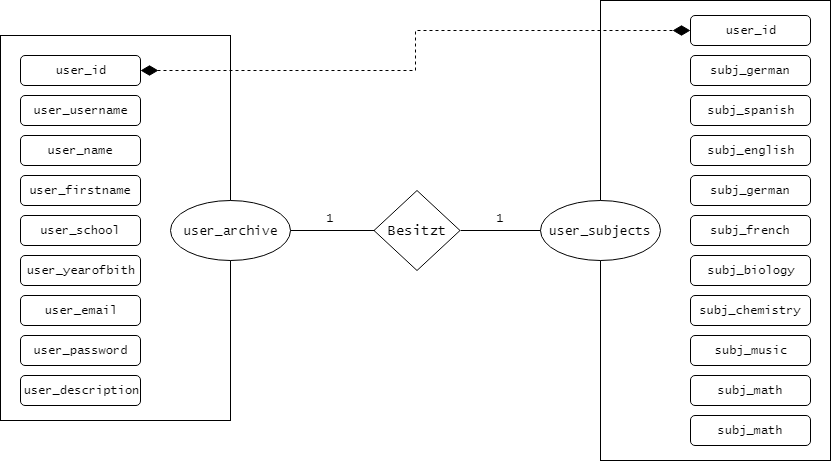
\includegraphics[scale=0.5]{ERM-Matura}
				%TODO BILD VON TABELLEN UND BESCHRIFTUNG
				
				\subsection{PHP Skripte} \label{ssec:PHP}
				DummyText...
					\subsubsection{Login}
					DummyText...
					\subsubsection{Registrierung}
					DummyText...
					\subsubsection{Änderungen via Einstellungen vom Client}
					DummyText...
					\subsubsection{Suchanfrage} \label{sssec:Suchanfrage}
					DummyText...
					
			\section{Firebase Realtime Server}
			DummyText...
				\subsection{Firebase}
				DummyText...
				\subsection{Firebasestruktur}
				DummyText...
		
		%Der Client
		\section{Client}
		DummyText...
			\subsection{Programmiersprache}
			DummyText...
			\subsection{Architektur des Clients}
			DummyText...
				\subsubsection{Klassenübersicht}
				DummyText...
			
			%Alle Module des Clients
			\subsection{Module}
				\subsubsection{Login Activity}
				DummyText...
				\subsubsection{Register Activity}
				DummyText...
				\subsubsection{Mainpage Activity}
				DummyText...
				\subsubsection{Settings Activity}
				DummyText...
				\subsubsection{Filter Activity}
				DummyText...
				\subsubsection{Searchresults Activty}
				DummyText...
				\subsubsection{Userprofile Activty}
				DummyText...
				\subsubsection{Chat Activity}
		
\newpage
\bibliography{literatur}	
	
\end{document}